\documentclass[hyperref={unicode=true}]{beamer}
\usepackage[T2A]{fontenc}
\usepackage[utf8]{inputenx}
\usepackage[russian]{babel}

\usepackage{multicol}

\usepackage[pgf]{dot2texi}
\usepackage{tikz}
\usetikzlibrary{shapes, arrows}

\usepackage{listings}
\usepackage{graphicx}

\usepackage{comment}

\title{Лекция 4. Язык Event-B}
\author{}
\date{}

\usetheme{Warsaw}

\AtBeginSection[] {
	\begin{frame}{Содержание}
		\tableofcontents[currentsection]
	\end{frame}
}
%\overfullrule=5pt

\begin{document}
	\begin{frame}{}
		\titlepage
	\end{frame}

    \begin{frame}{Цель лекции}
    Изучить язык Event-B и среду моделирования Rodin.
    \end{frame}

    \section{Введение}

	\begin{frame}{Почему Event-B}
    \begin{itemize}
		\item Сертификация по 4 уровню доверия к СЗИ требует 
		      разработать формальную модель управления доступом
			  и верифицировать ее с применением инструментальных
			  средств
		\item ГОСТ Р 59453.Х-2021 Защита информации. Формальная
		      модель управления доступом
		\item Event-B/Rodin - основные средства моделирования
			  и верификации формальных моделей управления доступом
	\end{itemize}
    \end{frame}

	\begin{frame}{Свойства Event-B/Rodin}
		\begin{itemize}
			\item формальный
			\item статически типизированный
			\item минималистичность
			\item математическая основа --- теория множеств
			\item наличие инструментальных средств для написания
			      моделей на Event-B и верификации (Rodin),
				  анимации (ProB) и др.
		\end{itemize}
	\end{frame}

	\begin{frame}{Дискретно-событийное моделирование}
		\begin{itemize}
			\item система обладает состоянием
			\item событие - воздействие на систему,
					система мгновенно дает отклик
					и может изменить свое состояние
			\item события упорядочены
			\item система может включать программы,
				  аппаратуру, внешнюю среду
		\end{itemize}
	\end{frame}

	\begin{frame}{Моделирование - это не программирование}
		Цель этой деятельности - не написание
		алгоритма/программы на "еще одном языке",
		а получение правильных требований к программе/системе:

		\begin{enumerate}
			\item Точные, недвусмысленные формулировки
			\item Абстракция (отсутствие лишних деталей $\rightarrow$ проще)
			\item Доказана непротиворечивость
			\item Возможна поэтапная разработка модели (добавление
			      информации небольшими порциями с постоянным
				  доказательством корректности)
		\end{enumerate}
	\end{frame}

	\begin{frame}{Основные элементы формального метода Event-B}
		\begin{itemize}
			\item статические свойства системы - `context`
			\item динамические свойства системы - `machine`
			\item формальная модель - множество контекстов и
			      последовательность машин
			\item контест может <<расширять>> другие контексты 
			\item машина может <<видеть>> несколько контекстов
			\item машина может <<уточнять>> другую машину
		\end{itemize}
	\end{frame}

	\begin{frame}[fragile]{Как это выглядит в Rodin}
		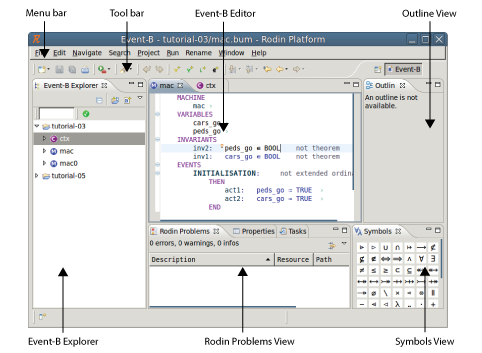
\includegraphics[scale=0.5]{rodin.png}
	\end{frame}

	\section{Синтаксис}

	\begin{frame}{Контекст}
		\begin{itemize}
			\item название контекста
			\item расширяемые контексты-предки
			\item несущие множества
			\item константы
			\item аксиомы/теоремы
		\end{itemize}
	\end{frame}

	\begin{frame}{Машина}
		\begin{itemize}
			\item название машины
			\item уточняемая абстрактная машина
			\item контексты
			\item переменные
			\item инварианты
			\item события (в т.ч. INITIALISATION)
		\end{itemize}
	\end{frame}

	\begin{frame}{Событие}
		\begin{itemize}
			\item название события
			\item уточняемое абстрактное событие
			\item параметры
			\item охранные условия
			\item действия
		\end{itemize}
	\end{frame}	

	\section{Типы данных и выражения}

	\begin{frame}{Простейшие типы данных}
		\begin{itemize}
			\item \texttt{INT}
			\item \texttt{NAT}
			\item \texttt{NAT1}
			\item \texttt{BOOL}
			\item несущие множества
		\end{itemize}
	\end{frame}

	\begin{frame}{Выражения --- общие положения}
		\begin{itemize}
			\item статически типизированы
			\item могут быть неопределены (пример: делят на 0),
			      есть wd-условие
			\item логика первого порядка: предикаты
			      и выражения синтаксически различаются
				  (значением переменной не может быть предикат,
				   но может быть функция)
		\end{itemize}
	\end{frame}

	\begin{frame}[fragile]{Логические выражения}
		\begin{itemize}
			\item константы \verb|TRUE|, \verb|FALSE|
			\item логические связки \verb|&|, \verb|or|,
			      \verb|=>|, \verb|<=>|, \verb|not|
			\item логические связи ленивые, при использовании
			      различных связок в одном выражении
			      скобки необходимы
			\item квантор всеобщности \verb|!|
			\item квантор существования \verb|#|
			\item сравнения \verb|=|, \verb|/=|, \verb|>|, ...
			\item принадлежность \verb|:|, \verb|/:|, \verb|<<|, ...
		\end{itemize}
	\end{frame}

	\begin{frame}[fragile]{Выражения с множествами}
		\begin{itemize}
			\item пустое множество \verb|{}|
			\item перечисление \verb|{1, 2, 3}|
			\item генератор \verb`{x * 2 | x : 1 .. 10}`
			\item целочисленные диапазоны (обе границы включаются) \verb|a .. b|
			\item теоретико-множественные операции \verb|\/|, \verb|/\|, \verb|\|
		\end{itemize}
	\end{frame}

	\begin{frame}[fragile]{Предопределенные функции и предикаты}
		\begin{itemize}
			\item предикат как выражение типа \texttt{BOOL} \verb|bool(predicate)|
			\item конечность множества \verb|finite(set)|
			\item размер множества \verb|card(set)|
			\item равенство объединению непересекающихся множеств
			      \verb|partition(set, set1, set2, ..., setN)|
		\end{itemize}
	\end{frame}

	\begin{frame}[fragile]{Пары и отношения}
		\begin{itemize}
			\item пара \verb`a |-> b`
			\item декартово произведение \verb|A ** B|
			\item множество подмножеств \verb|POW(A)|, \verb|POW1(A)|
			\item произвольное отношение \texttt{A <-> B}
			\item тотальное отношение \verb`A <<-> B`
			\item сюръективное отношение \verb`A <->> B`
			\item тотальное сюръективное отношение \verb`A <<->> B`
		\end{itemize}
	\end{frame}

	\begin{frame}[fragile]{Операции над отношениями}
		\begin{itemize}
			\item область определения (домен) \verb|dom(relation)|
			\item область значений \verb|ran(relation)|
			\item проекция \verb|relation[set]|
			\item оставить только поддомен \verb`set <| relation`
			\item убрать поддомен \verb`set <<| relation`
			\item оставить только значения \verb`relation |> set`
			\item убрать значения \verb`relation |>> set`
		\end{itemize}
	\end{frame}

	\begin{frame}[fragile]{Функции}
		Функция --- это детерминированное подмножество отношения.

		\begin{itemize}
			\item множество тотальных функций \verb|A -> B|
			\item множество частичных функций \verb|A +-> B|
			\item применение \verb|function(arg)|
		\end{itemize}
	\end{frame}

	\begin{frame}[fragile]{Действия}
		\begin{itemize}
			\item одиночное \verb|x := E|
			\item множественное \verb|x1, x2, ..., xN := E1, E2, ..., EN|
			\item замена пары в отношении \verb|x(F) := E|
			\item неявное одиночное  \verb`x :| before-after-predicate with x and x'`
			\item неявное множественное
			      \verb`x1, ..., xN :| b-a-p with x1, ..., xN, x1', ..., xN'`
			\item неявный выбор из непустого множества \verb`x :: set`
		\end{itemize}
	\end{frame}

	\section{Семантика}

	\begin{frame}{Функционирование машины}
		\begin{enumerate}
			\item состояние машины --- значения всех переменных
			\item событие --- переход из одного состояния в другое
			\item событие может иметь параметры
			\item переход возможен, только если истинны
			      все охранные условия
			\item в этом случае выполняются все действия
			\item действия одного события выполняются одновременно
			\item начальное состояние --- результат события \texttt{INITIALISATION}
		\end{enumerate}
	\end{frame}

	\begin{frame}{Корректно определенная машина/контекст}
		\begin{enumerate}
			\item \texttt{WD}: нет неопределенных выражений
			\item \texttt{INV}: не нарушены инварианты
			\item \texttt{THM}: не нарушены теоремы
			\item \texttt{FIS}: неявные действия разрешимы
			\item \texttt{GRD}, \texttt{SIM}, \texttt{EQL}:
			      уточнение корректно
		\end{enumerate}

		Rodin генерирует условия верификации для формального
		доказательства, что машина корректно определена.
	\end{frame}


\end{document}

